% Copyright 2019 Clara Eleonore Pavillet

% Author: Clara Eleonore Pavillet
% Description: This is an unofficial Oxford University Beamer Template I made from scratch. Feel free to use it, modify it, share it.
% Version: 1.0

\documentclass{beamer}
\usepackage{verbatim}
\newenvironment{metaverbatim}{\verbatim}{\endverbatim}
% Load Packages
\usepackage[utf8]{inputenc}
\usepackage{xcolor}
\usepackage{tikz}
\usetikzlibrary{positioning,calc}
\usepackage{graphicx}
\usepackage{hyperref}
\usepackage{amsmath}
\usepackage{listings}
\usepackage{fontawesome}

% Define Commands
\newcommand*{\ClipSep}{0.06cm} %To adjust footer logo
\newcommand{\E}{\mathrm{e}\,} %\def\I{e} % used to defined e for exp(x), see later what it should be
\newcommand{\ud}{\mathrm{d}}
\lstset{numbers=left, numberstyle=\tiny, stepnumber=1,firstnumber=1,breaklines=true,
    numbersep=5pt,language=Python,
    stringstyle=\ttfamily,
    basicstyle=\footnotesize, 
    showstringspaces=false
}

\usetheme{Madrid}

\title{Dolo for absolutely beginners}
% \titlegraphic{
\includegraphics[width=2cm]{Theme/Logos/OxfordLogoV1.png}}
\author{Euiyoung Jung}
\institute{PSE}
\date{} %\today

\begin{document}

{\setbeamertemplate{footline}{} 
\frame{\titlepage}}

% \section*{Outline}\begin{frame}{Outline}\tableofcontents\end{frame}

\begin{frame}{Introduction}
    \begin{itemize}
        \item If you do not have any prior knowledge about \textit{Dolo} and try to follow the instruction provided by the program developer, you will almost always encounter error messages from the very beginning. 
        \item For example, you can find the following instruction in order to verify whether installation is done well or not. 
        \item Unfortunately, it will not work! It is because the default \textit{YAML} page is expired.
    \end{itemize}
    \end{frame}
\begin{frame}
     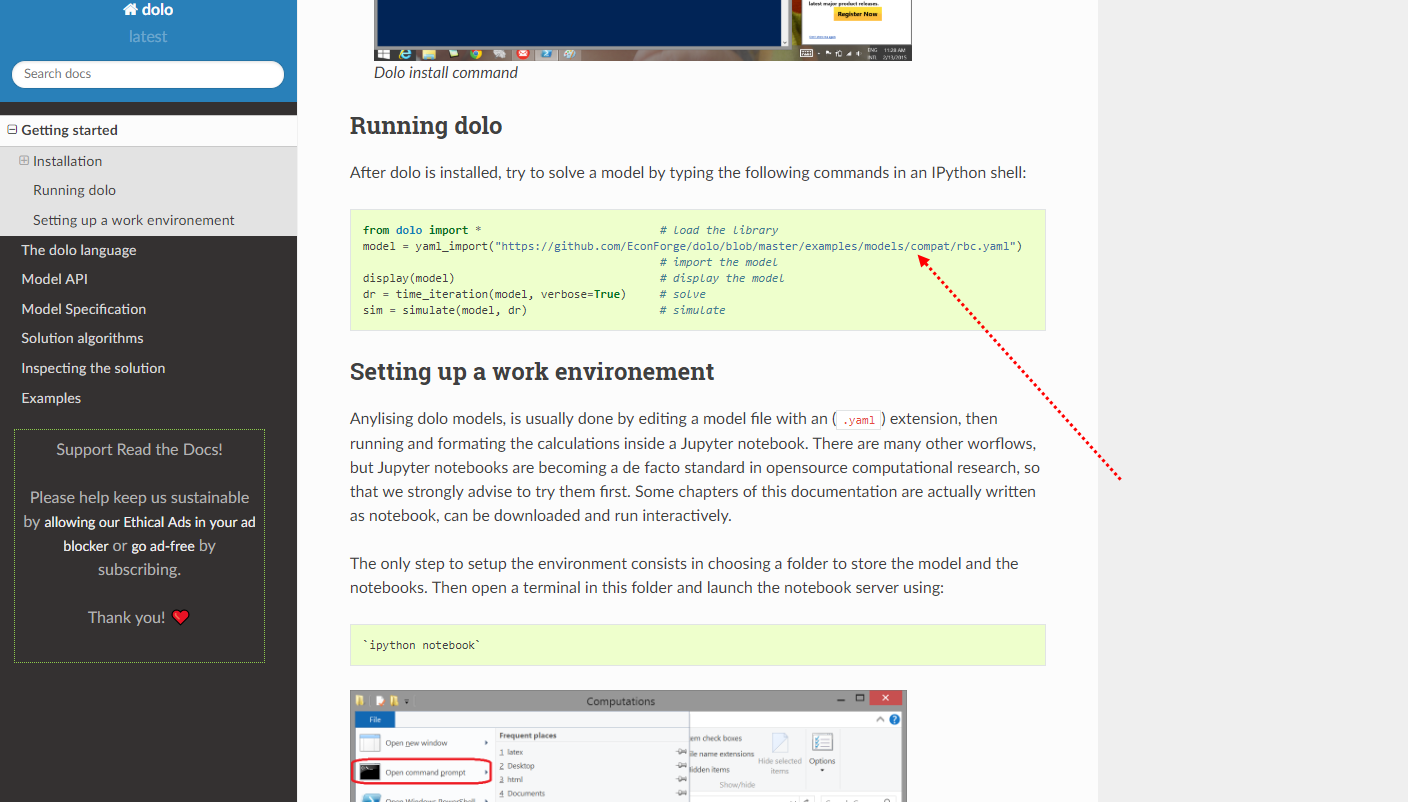
\includegraphics[width=12cm, height= 8cm]{dolo4.png} 
\end{frame}
\begin{frame}
    \begin{itemize}
    \item Instead of using the url in the manual, copy and paste this one: \url{https://raw.githubusercontent.com/EconForge/dolo/master/examples/models/rbc.yaml}  
    \item Your installation might be done well if \textit{Dolo} is running without error messages, once you try with url given above. 
        \item In order to write down your own model, the first step you have to do is making a github repository.
        \item Note: You have to make your repository \textbf{public}. Otherwise, your local python like \textit{Jupyter notebook} cannot call your \textit{YAML} file. 
        \item Let's start from basic housechores step by step. 
    \end{itemize}
\end{frame}
  \begin{frame}{Making a Github repository}
           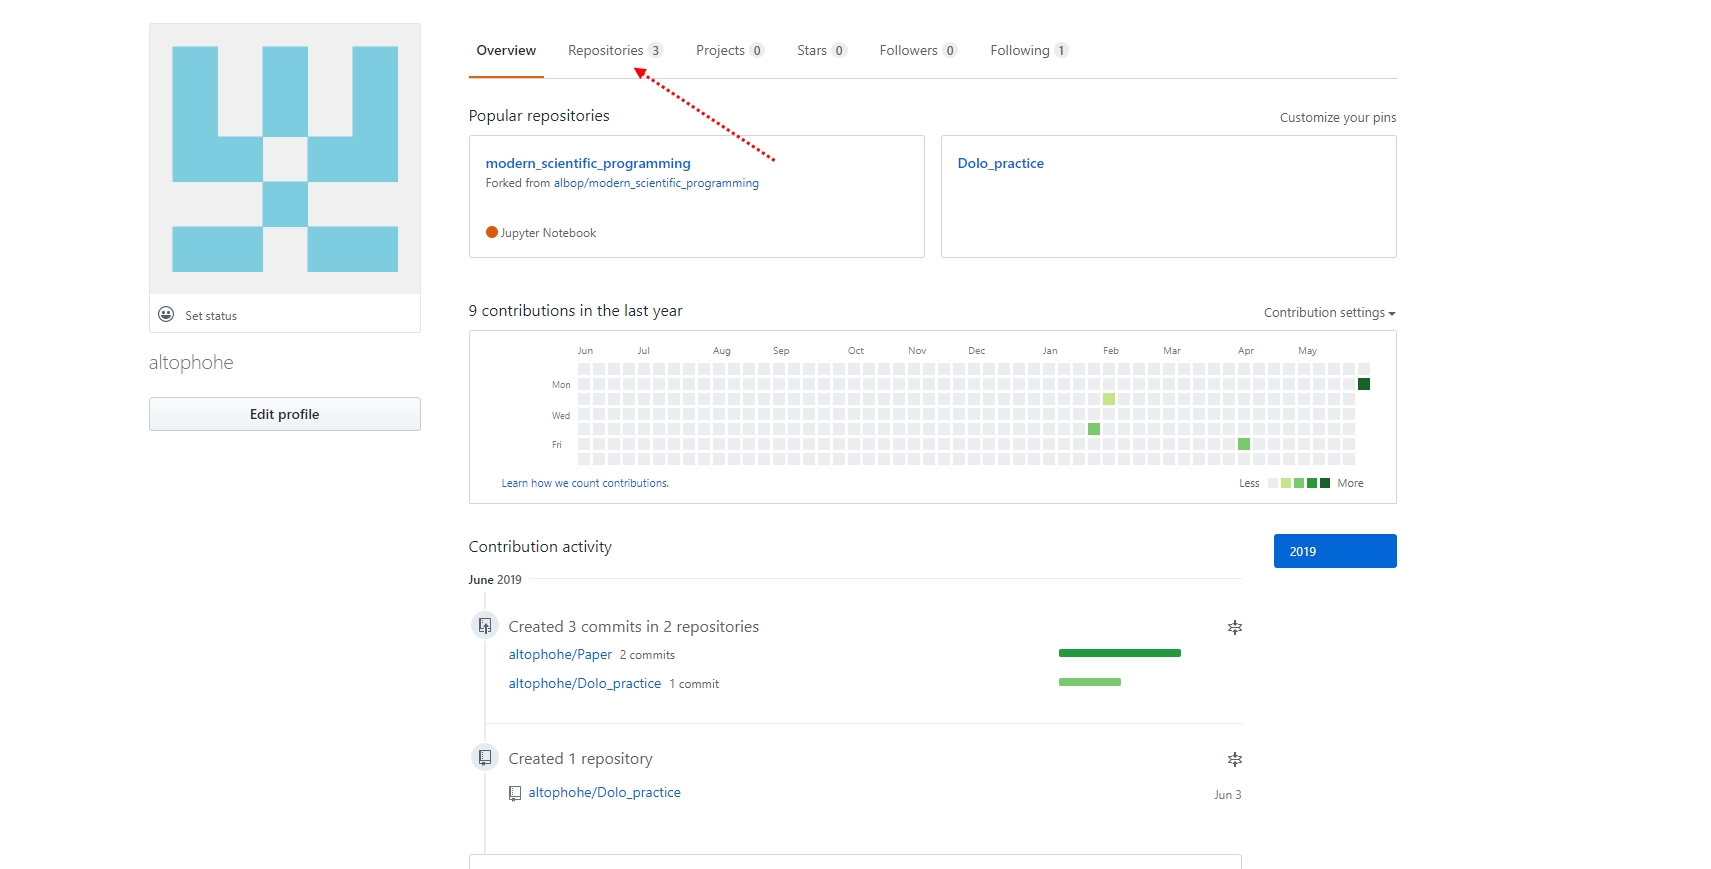
\includegraphics[width=12cm, height= 8cm]{dolo1.jpg} 
    \end{frame}
    \begin{frame}{Making a Github repository}
           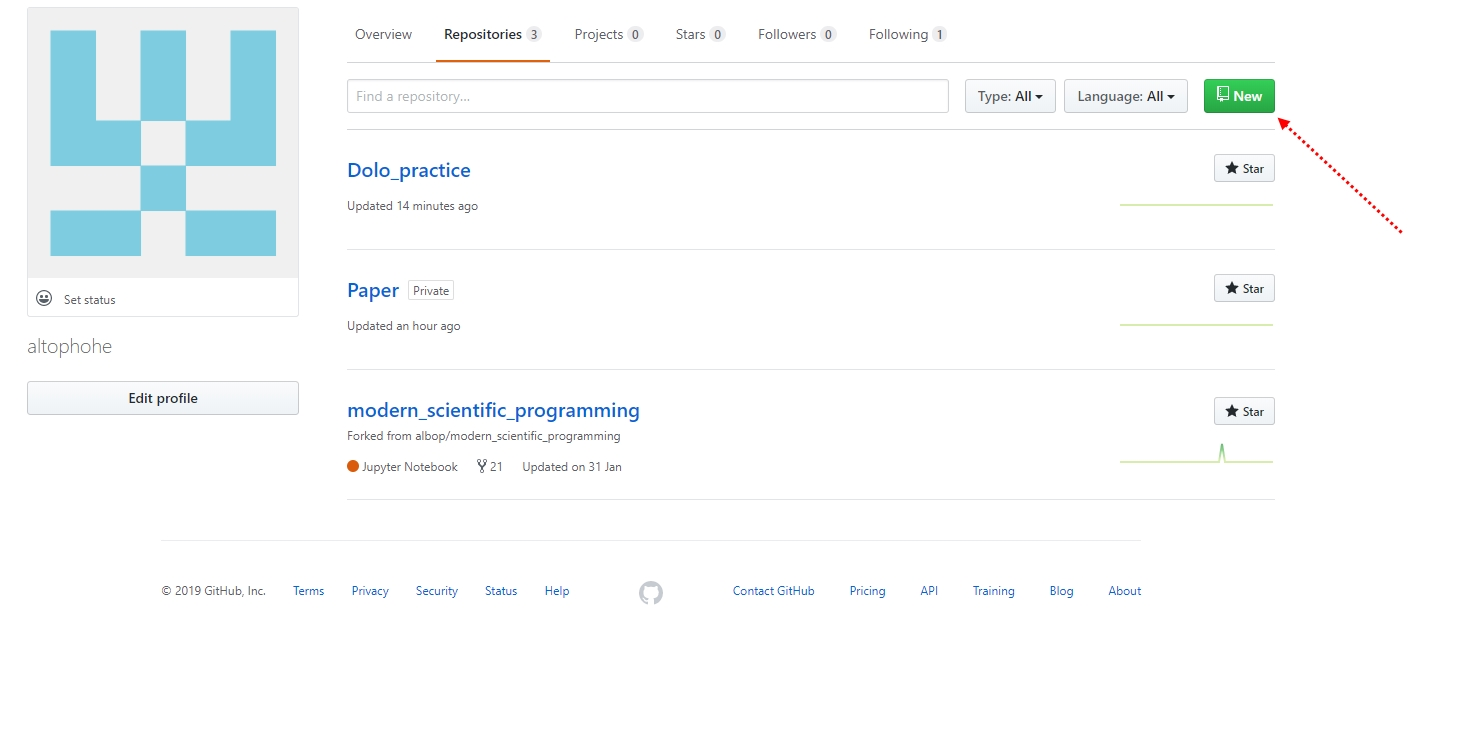
\includegraphics[width=12cm, height= 8cm]{dolo2.jpg} 
    \end{frame}
     \begin{frame}{Making a Github repository}
           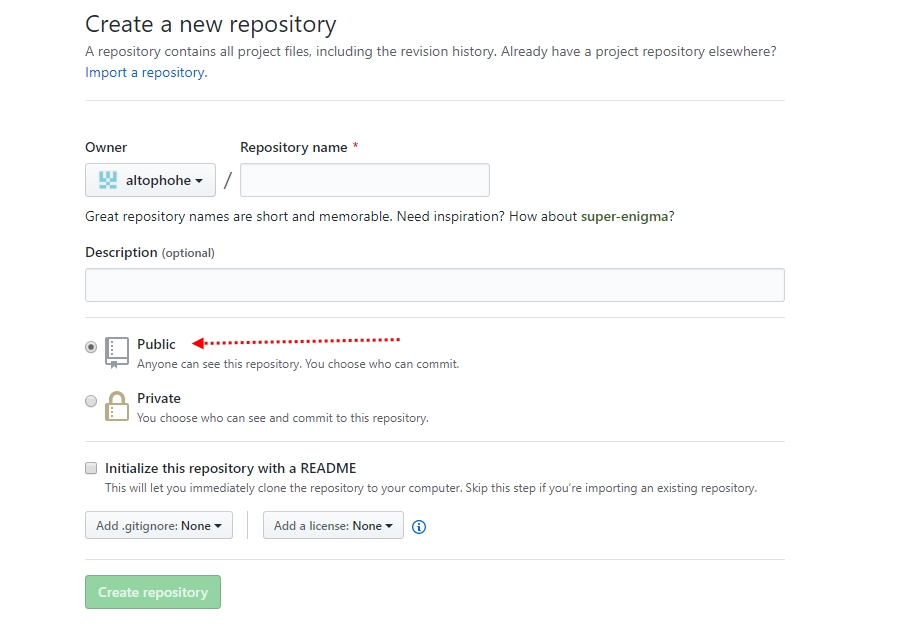
\includegraphics[width=12cm, height= 8cm]{dolo3.jpg} 
    \end{frame}
  
\begin{frame}{Making a Github repository}
    \begin{itemize}
    \item If you could manage to do all steps so far, now you made your own Github repository. 
    \item You can write your own \textit{YAML} file which would be the the backbone of Dolo computation.
        \item The easiest way for a beginner is utilizing examples provided by the developer. You can find several examples from Pablo Winant's Github repository:\\
        \url{https://github.com/EconForge/dolo/tree/master/examples/models}
        \item The Dolo language and the way to write down the model can be found at \url{https://dolo.readthedocs.io/en/latest/}
        \item Writing an \textit{YAML} model file in your own repository may not be easy. Let's start from Pablo Winant's example. 
    \end{itemize}
\end{frame}
    \begin{frame}{Dolo examples}
 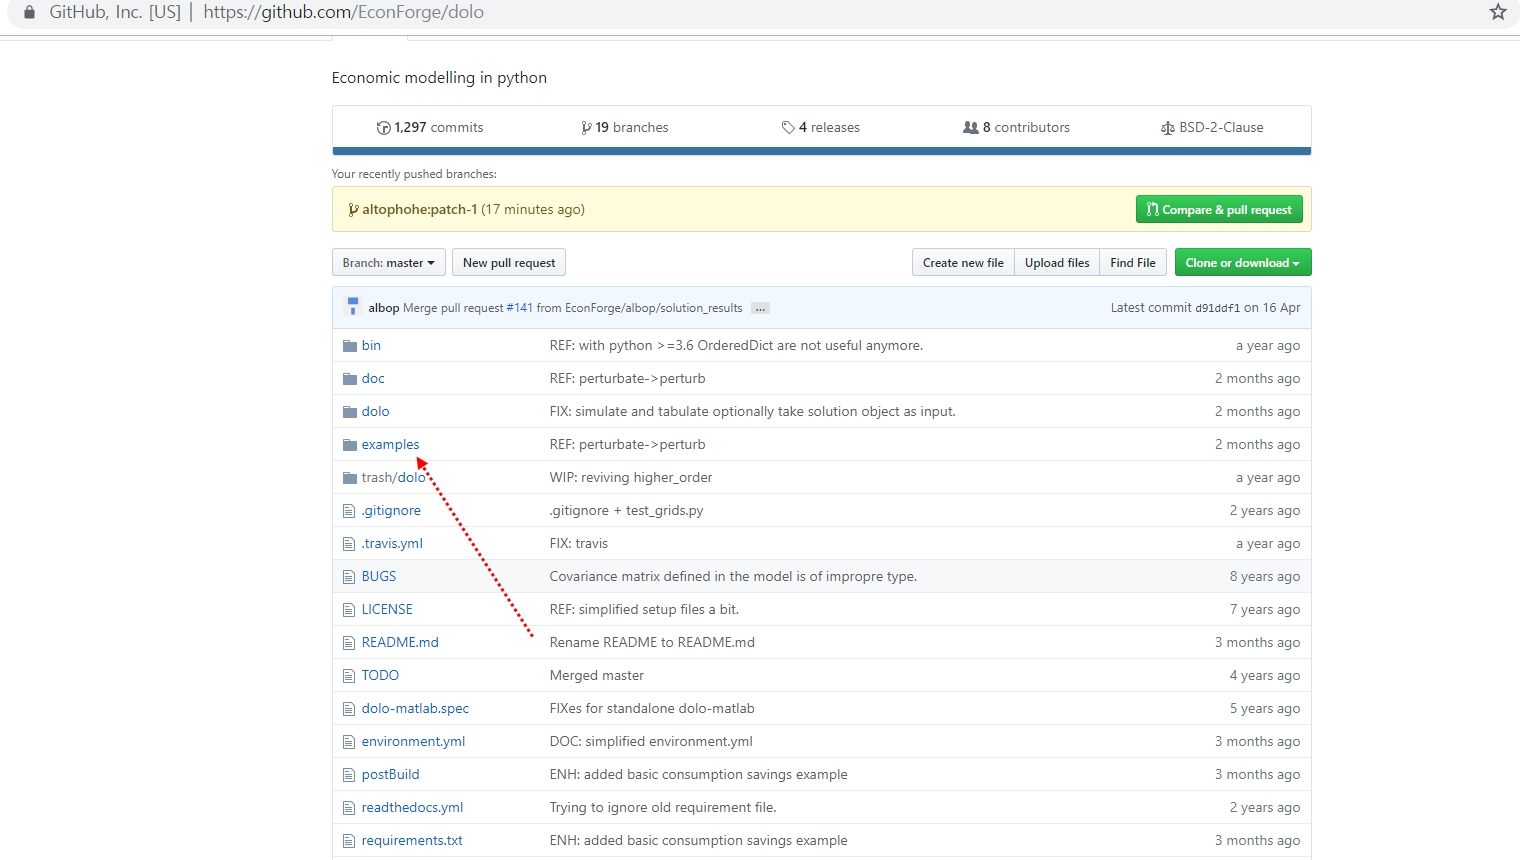
\includegraphics[width=12cm, height= 8cm]{dolo5.jpg}
    \end{frame}
    \begin{frame}{}
         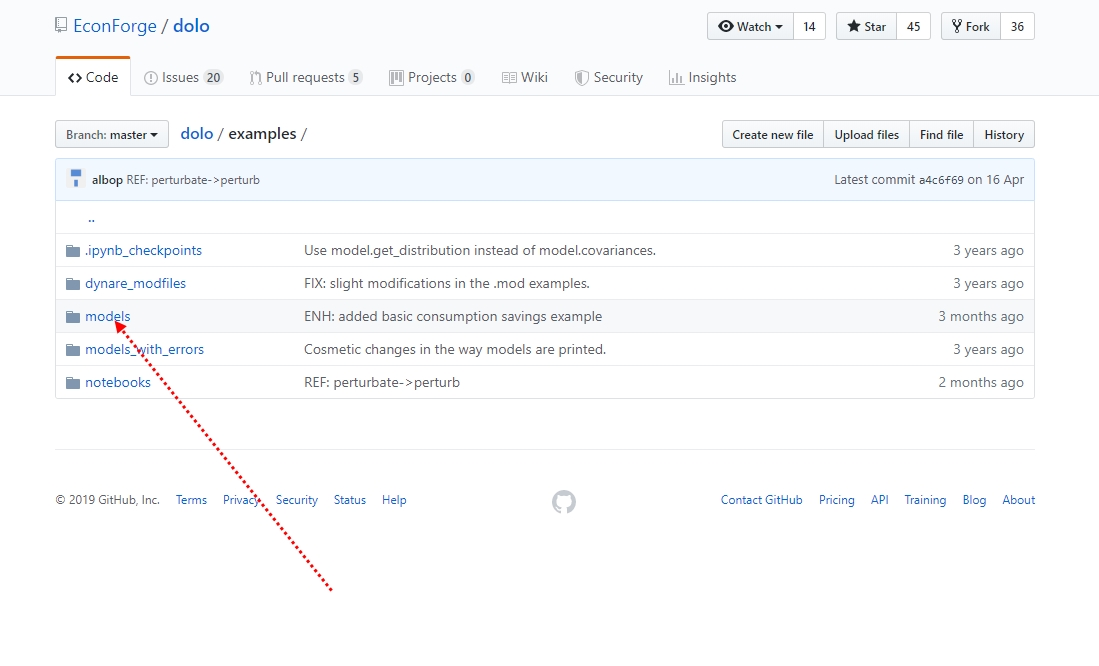
\includegraphics[width=12cm, height= 8cm]{dolo6.jpg}
    \end{frame}
    \begin{frame}{Dolo examples}
        \begin{itemize}
            \item From Pablo's github repository, you can copy and paste any \textit{YAML} model file. 
            \item If you make an \textit{YAML} file in your own repository, then you have to be able to run it in your local python. 
            \item To call the model file, you have to get the raw content of files stored in Github. This can be done as follows. 
        \end{itemize}
    \end{frame}
     \begin{frame}{}
         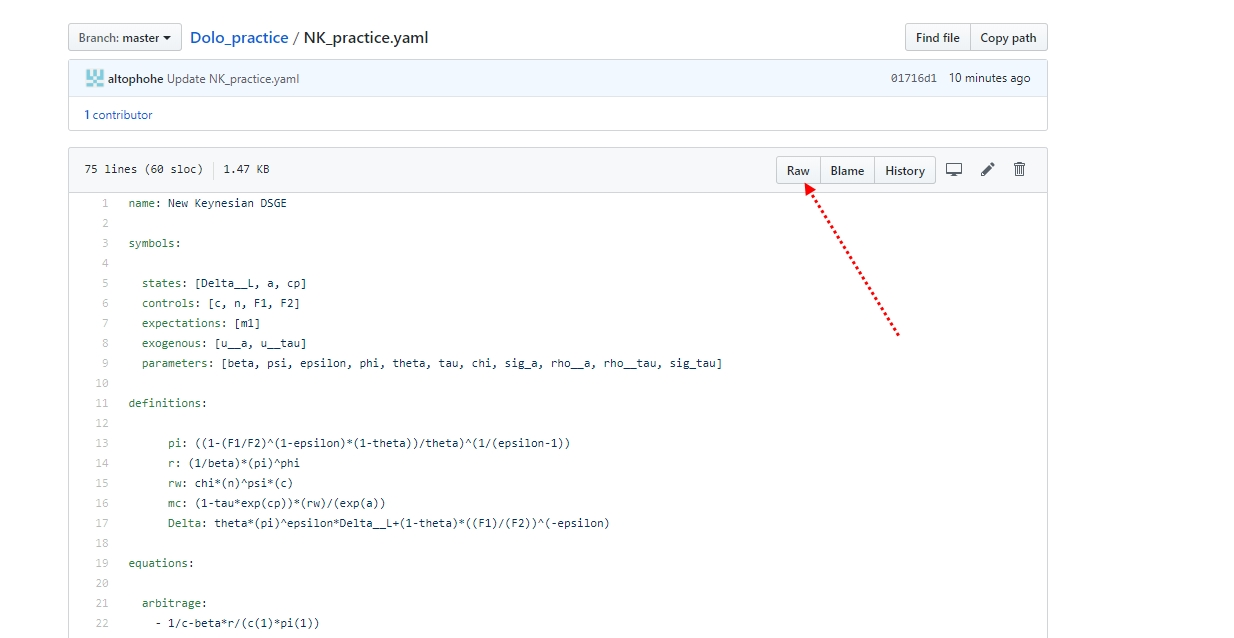
\includegraphics[width=12cm, height= 8cm]{dolo8.jpg}
    \end{frame}
     \begin{frame}{}
         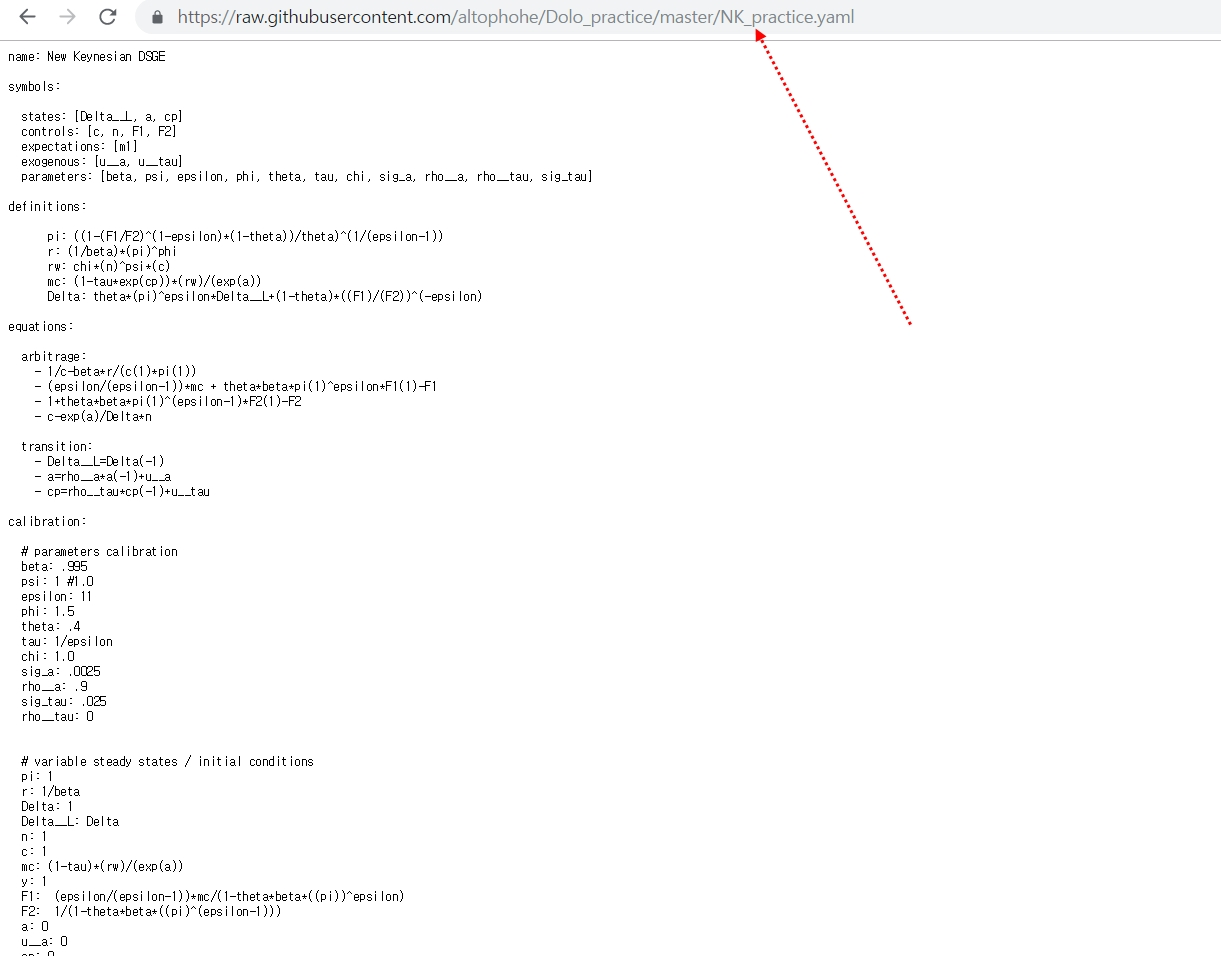
\includegraphics[width=12cm, height= 8cm]{dolo9.jpg}
    \end{frame}
\begin{frame}{Dolo examples}
\begin{itemize}
  
    \item Type following commands on your \textit{Jupyter notebook}:\\
    
    filename = ('\textit{your yaml raw file address here}')\\
    model = yaml\_ import(filename)\\
    display(model)  

\item If you write a model file without error and dolo is installed well in your computer, you would see that Jupyter displays the model. 
\item If you can manage to get here, you are basically ready to do further works such as impulse-response, simulations, projection and so on.
\item The key and most tricky part for your own project may be to write your model file properly. Once you can run your model, thanks to dolo's built-in commands, extended works can be easily conducted as if \textit{Dynare} does. 
\end{itemize}
\end{frame}

\begin{frame}{Model}
    \begin{itemize}
        \item I try to solve a simplified RBC model with a search and matching friction in the labor market and costly separation. 
        \item Only 1 exogenous shock is in place: TFP
        \item Idiosyncratic match specific productivity shock follows Pareto distribution, defined over the interval $[1, \infty]$
        \item Due to this lower bound, the occasionally binding constraint is likely to bind(no-separation corner solution). As a result, the standard perturbation method is not enough to accurately solve the model.   
        \item I skip explaining the model in detail as it is not our main interest, but just enumerate the equilibrium conditions. 
    \end{itemize}
\end{frame}
\begin{frame}{Few remarks when writing a model}
    \begin{itemize}
        \item Github Raw file is not updated in real time, but you need to wait for a few seconds. So, when you change the model and apply the url to your python code, the changed yaml version may not be used yet. So, you have to check it first. 
        \item As other python coding practice, indentation seems to be important. Do not make any unnecessary space in your code. 
        \item When using lambda for your parameter or variable, you should be careful as lambda is an integral python command declaring a local function. I highly recommend  to use a different name for your lambda parameter (or variable) .  \item I don't know the reason exactly, but I get an error when I write some comment in the code using sharp mark. 
        
    \end{itemize}

\end{frame}
\begin{frame}{Few remarks when writing a model}
    \begin{itemize}
       \item In the manual, it is said that contemporaneous endogenous variables can be written in \textit{direct response} section. However, I also get the error message. Once I put those equations in the definition section, the code seems to run. \item When writing the equations, it seems that you have to write those in accordance with the order of variable declaration. For example, if you declare the state variable as [k,A], then the transition equation for k should be written first than A.  
    \end{itemize}
\end{frame}
\begin{frame}{Model}
    \begin{align}
    &-T-\mu_tA_t\bar{a}_t-\lambda_t+e_{\bar{a},t}=0\\
    & -\mu_tA_t\hat{a}_t-\lambda_t+e_{\hat{a},t}=0\\
    &F_t=1-(\frac{a_L}{\bar{a}_t})^{\alpha}\\
    &\hat{F}_t=1-(\frac{a_L}{\hat{a}_t})^{\alpha}\\
    &E(\bar{a}_t)=\frac{\alpha}{\alpha-1}(\frac{a_L}{\bar{a}_t})^{\alpha-1}\\
    &E(\hat{a}_t)=\frac{\alpha}{\alpha-1}(\frac{a_L}{\hat{a}_t})^{\alpha-1}
      \end{align}
      where $e_{\bar{a},t}$ and $e_{\hat{a},t}$ are the KKT Lagrange multipliers, satisfying $e_{\bar{a},t}=0$ iff $\bar{a}_t=a_L$. $\hat{a}_t$ case is similar. $\lambda$ above is named as $x$ in my \textit{YAML} file. 
\end{frame}

\begin{frame}{Model}
    \begin{align}
     &\tilde{u}_t=u_{t-1}+F_tn_{t-1}\\
     &\Theta\frac{Y_t}{n_t}=q_t(\mu_tA_tE(\bar{a}_t)+\lambda_t(1-\hat{F}_t))\\
    &n_t=(1-F_t)n_{t-1}+(1-\hat{F}_t)M_{t}\\
    &M_t=\chi \tilde{u}_{t}^\gamma v_{t}^{1-\gamma}\\
    &u_t=1-n_t\\
    &Y_t=A_t(n_{t-1}E(\bar{a}_t)+M_tE(\hat{a}_t))\\
    &q_t= \frac{M_t}{v_t} \\
    &f_t=\frac{M_t}{\tilde{u}_{t}}\\
    &\theta_t=\frac{v_t}{\tilde{u}_t}
    \end{align}
\end{frame}
\begin{frame}{Model}
    \begin{align}
      &w_t=w(\frac{Y_t}{Y})^{\gamma_w}\\
    &b_t=\tilde{r}w_t\\
    &C_t=w_tn_t+b_tu_t\\
     &C_t+C_t^e=(1-\Theta(\frac{ v_t}{n_t})-\frac{TF_tn_{t-1}}{Y_t} -\Phi)Y_t\\
    &1= \beta E_t\left[Q_t\frac{C_{t+1}^{-\sigma}}{C_t^{-\sigma}}\right]\\
    & \lambda_t=-w_t+\beta E_t[-TF_{t+1}+\mu_{t+1}A_{t+1}Ea_{t+1}+(1-F_{t+1})\lambda_{t+1}]\\  & A_t=\textbf{A}e^{\tilde{A}_t}\\
    & \tilde{A}_t=\rho_A \tilde{A}_{t-1}+e_t^A
      \end{align}
\end{frame}
\begin{frame}{Model}
    \begin{itemize}
        \item \textit{YAML} model file can be written such that:
    \end{itemize}
\end{frame}
\end{document}
